\documentclass{beamer}
\mode<presentation> {
  \usetheme{Boadilla}
  \usecolortheme{dolphin}
  % \setbeamertemplate{footline}
  \setbeamercovered{transparent}
  \setbeamertemplate{caption}{\raggedright\insertcaption\par}
}
\usepackage[utf8]{inputenc}
\usepackage[T1]{fontenc}
\usepackage[english]{babel}
\usepackage{graphicx}
\usepackage{caption}
\usepackage{hyperref}
\captionsetup[figure]{labelformat=empty}
\begin{document}
\title{stv-vwsozoekseep@wu.ac.at}
\author{Student Representatives Economics}
\date{2018/10/01}
\begin{frame}  
  \frametitle{Welcome to WU! Welcome to the Master's in Economics!}
  \uncover<1>{
  \begin{block}{About us}
   \begin{itemize}
      \item Your representation
      \item Economics, Socio-Economics and Socioecological Economics and Policy 
      \item Elections next year!
    \end{itemize}
   \end{block}
 }
 \uncover<2>{
    \begin{block}{Elections}
      \begin{itemize}
       \item You can vote on 3 levels:
         \begin{enumerate}
         \item Federal level: ``Bundesvertretung''
         \item University level: ``Hochschulvertretung''
         \item Program level \\(i.e. Master's Economics): ``Studienvertretung'' $\Rightarrow$ that's us!
         \end{enumerate}
         We are from the VSST\"O (Democratic Socialists). 
      \end{itemize}
   \end{block}
}
\end{frame}

\begin{frame}
  \frametitle{Your representatives}
  \centering
  \begin{figure}
    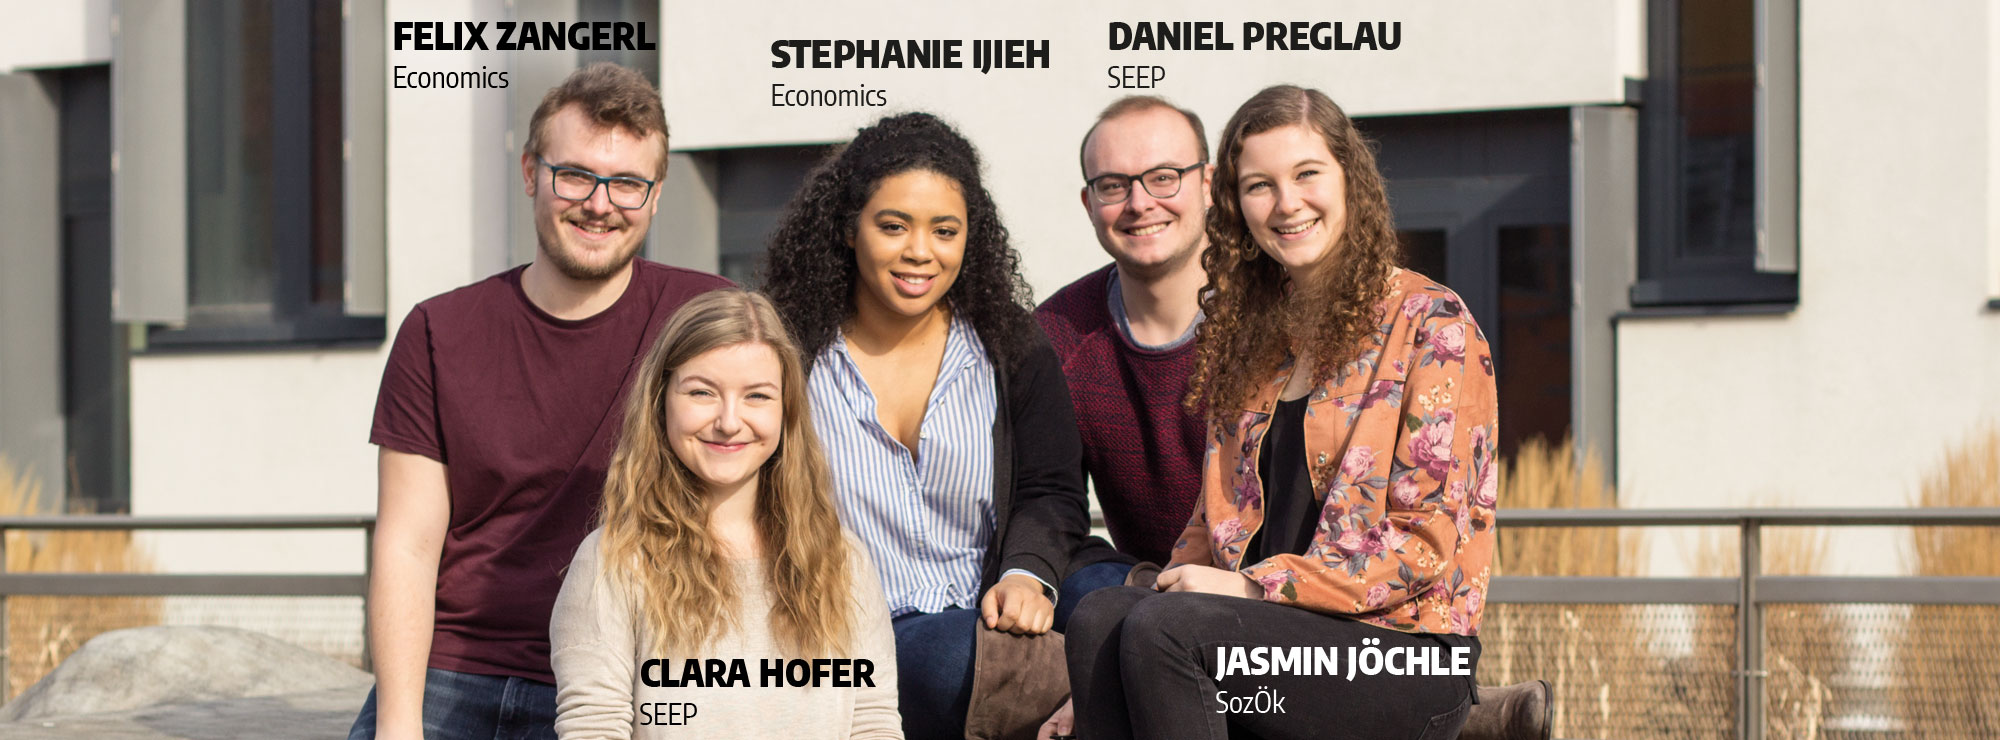
\includegraphics[scale = 0.16]{team} 
    \caption{Daniel, Sarah, Bernhard \\ Veronika \& Camila}
  \end{figure}
\end{frame}

\begin{frame}
  \frametitle{What we do}
  \begin{block}{Representation}
    \begin{itemize}
    \item Senate \& Committees \\
      (e.g. academic calendar, nomination of professors, $\dots$)
    \item Legal questions
    \item Disputes
    \end{itemize}
  \end{block}
  \begin{block}{Networking}
    \begin{itemize}
    \item Weekly gatherings: \textbf{You are invited!}
    \item Events  
    \end{itemize}
  \end{block}
  \begin{block}{Education}
    \begin{itemize}
    \item Book Club (``Lesekreis'')
    \item Lectures \& Courses
    \item R-Tutorials \\
      \href{https://gitlab.com/r-students-WU/tutorial-winter-2018}{Link: gitlab}
    \end{itemize}
  \end{block}
\end{frame}

\begin{frame}
  \frametitle{Student Newspaper}
  \begin{itemize}
  \item ``Standpunkte''
  \item Contact: \href{mailto:standpunkte.zeitung@gmail.com}{standpunkte.zeitung@gmail.com}
    \href{https://www.wu.ac.at/economics/vw-zentrum/standpunkte/}{Link: Standpunkte}
  \item Book reviews, topics you are interested in
  \item Previous articles and topics:
    \begin{itemize}
    \item ``EU and UK – A complicated relationship that will end in a divorce''
    \item ``How to switch back to “boring monetary policy“ without being trapped at the zero lower bound''
    \item Climate change
    \item Pluralism in Economics
    \item Various ``schools'' in Economics
    \end{itemize}
  \end{itemize}
\end{frame}
\begin{frame}
  \frametitle{Contact us!}
  \begin{itemize}
  \item Facebook: \href{https://www.facebook.com/vwsozoekseep/}{www.facebook.com/vwsozoekseep/}
  \item E-mail: \href{mailto:stv-vwsozoekseep@wu.ac.at}{stv-vwsozoekseep[at]wu.ac.at}
  \item Website: \href{https://stv-vw-sozoek-seep.github.io/website/}{stv-vw-sozoek-seep.github.io/website/} \\
    Short: \href{https://tinyurl.com/vwsozoekseep}{tinyurl.com/vwsozoekseep}
  \item Gitlab: \href{https://gitlab.com/r-students-WU}{gitlab.com/r-students-WU}
  \end{itemize} 
\end{frame}
\end{document}
%%% Local Variables:
%%% mode: latex
%%% TeX-master: t
%%% End:
